\documentclass{article}
\usepackage[x11names]{xcolor}
\usepackage{pgfplots}
\usepgfplotslibrary{fillbetween}
\pgfplotsset{compat=1.8}
\usetikzlibrary{calc}	

\begin{document}

%\foreach \a in {0, 45, 90}{
%\begin{tikzpicture}
%\begin{axis}[view={\a}{0},
%xlabel = $x$,
%ylabel = $y$,
%zlabel = $z$,
%zlabel style = {rotate=90}]
%\addplot3[surf,y domain=-2*pi:2*pi,] {sin(deg(y))};
%\def\x{1}
%\foreach \joo in {-pi, -pi/2, 0, pi/2, pi}{
%\def\y{pi}
%	\pgfmathsetmacro{\z}{{sin(deg(\y))}}
%	\pgfmathsetmacro{\pituus}{{sqrt(cos(deg(\y))^2+1)}}
%	\coordinate (A) at (axis cs: {\x}, {\y}, {\z});
%	\coordinate (B) at (axis cs:{\x},{\y-(cos(deg(\y)))},{\z+1/\pituus});
%	\draw[very thick,->](A)--(B);
%}
%\end{axis}
%\end{tikzpicture}
%}

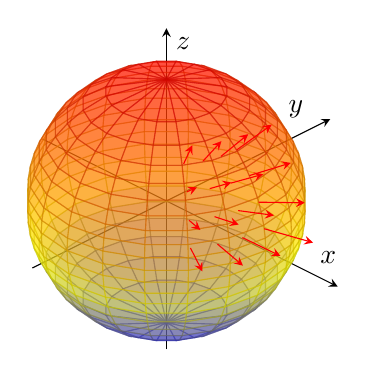
\begin{tikzpicture}
    \begin{axis}[%
        axis equal,
        width=10cm,
        height=10cm,
        axis lines = center,
        xlabel = {$x$},
        ylabel = {$y$},
        zlabel = {$z$},
        ticks=none,
        ymin = -1.1,
        ymax=1.4,
        zmax=1.2,
        enlargelimits=0.1,
        view/h=45,
        scale uniformly strategy=units only,
    ]
    \addplot3[
        surf,
        opacity = 0.5,
        samples=21,
        domain=-1:1,y domain=0:2*pi,
        z buffer=sort]
    ({sqrt(1-x^2) * cos(deg(y))},
     {sqrt( 1-x^2 ) * sin(deg(y))},
     x);
     \addplot3[samples=4,quiver,-stealth,%opacity=0.1,
      domain=0:35,domain y=10:45,point meta=1,
      quiver={
        u={x/sqrt((x)^2+(y)^2+(z)^2)},
        v={y/sqrt((x)^2+(y)^2+(z)^2)},
        w={z/sqrt((x)^2+(y)^2+(z)^2)},
        colored,scale arrows=0.5}]
      ({cos(y)*cos(x)},{-cos(y)*sin(x)},{sin(y)});
    %}

    \end{axis}
\end{tikzpicture}

\end{document}